%Included for Gather Purpose only:
%input "auth.bib"
\documentclass[times, 10pt,twocolumn]{article}
\usepackage{latex8}
\usepackage{times}

% support for sub-figures
\usepackage{subfigure}
% floating/wrapping support
\usepackage{floatflt}
\usepackage{epsfig}

\pagestyle{empty}

\begin{document}

\title{Authentication in Stealth Distributed Hash Tables}

\author{
Andrew MacQuire \hspace{1em}
Andrew Brampton \hspace{1em}
Idris A. Rai \hspace{1em}
Nicholas J. P. Race \hspace{1em}
Laurent Mathy\\
Computing Department \\
Lancaster University \\
\{macquire,brampton,rai,race,laurent\}@comp.lancs.ac.uk\\
}

\maketitle
\thispagestyle{empty}

\begin{abstract}
Most existing DHT algorithms assume that all nodes have equal
capabilities. This assumption has previously been shown to be untrue in
real deployments, where the heterogeneity of nodes can actually have a
detrimental effect upon performance. In this paper, we acknowledge that
nodes on the same overlay may also differ in terms of their
trustworthiness. However, implementing and enforcing security policies
in a network where all nodes are treated equally is a non-trivial task.
We therefore extend our previous work on Stealth DHTs to consider the
differentiation of nodes based on their trustworthiness rather than
their capabilities alone. %Particularly, we discuss how a suitable
%Public Key Infrastructure can be used in conjunction with a Stealth DHT
%to separate nodes into multiple classes with differing privileges, thus
%greatly improving the security properties of the network. We also
%consider the various implementation issues involved and discuss
%possible solutions.
\end{abstract}

\Section{Introduction}
\label{sect-intro}

Distributed Hash Tables (DHTs) have been shown to be a useful form of
decentralised, structured peer-to-peer
overlay~\cite{Rowstron01Pastry}\cite{Stoica01Chord}\cite{Zhao01Tapestry}\cite{Ratnasamy01Scalable}.
They allow for the provision of simple hash table functionality -- that
is, the ability to \emph{put} and \emph{get} pieces of data indexed via
hash codes -- across multiple nodes in a scalable and resilient
fashion. Primarily, DHTs have been used as location substrates for many
varied applications, such as large-scale file
storage~\cite{Druschel01PAST}\cite{Dabek01Wide}\cite{Kubiatowicz00OceanStore}
and multicast~\cite{Rowstron01SCRIBE}\cite{Zhuang01Bayeux}, amongst
others.

Theoretically, most DHTs consist of numerous nodes which organise
themselves and behave in a well defined manner. Each node is
associated with a unique identifier (ID), randomly selected from a
large, sparsely-populated address space. When an object is
\emph{put} into a DHT, its contents are hashed in some way as to
produce an identifier which also maps into this address space. The
originating node then routes the object to the local node that it
knows to have the closest-matching identifier. If the recipient
knows of an even closer node, it then forwards the data on.
Eventually, the object reaches a node which does not know of any
closer match. This node is considered the final destination, and
must then take responsibility for the storage and/or any other
handling of the object. Any individual who then wishes to \emph{get}
the same object at a later date can then do so based on the
knowledge of the object's hash alone, as any message routed to the
same hash should arrive at the same node that the object originally
reached. Of course, this can only occur if all nodes follow the DHT
protocol correctly.

Unfortunately, in a real-world deployment it would be na\"ive to assume
that all nodes can be relied upon to conform to any prescribed
behaviour. Without appropriate security policies in place, numerous
problems may exist for public DHTs. For instance, a malicious node may
examine, alter or deliberately drop messages passed through it
(\emph{i.e.} a sniffing, man-in-the-middle or denial of service
attack). The ability to inject unsolicited messages into the DHT, or to
alter those in transit, also allows untrustworthy nodes to corrupt the
routing tables of others. Possible consequences of such actions could
be legitimate nodes being denied service, or malicious nodes improving
their standing on the network at the expense of others. In terms of
content in the DHT, if all nodes are allowed to perform \emph{put}
operations, then the pollution of the system with unwanted
or illegal data may become an issue. %Furthermore, existing DHT
%algorithms used in peer-to-peer networks provide ideal environments for
%users to infringe intellectual property law because they allow users to
%easily duplicate copyrighted works or distribute illegal content. This
%is a major factor that hinders commercial use of existing DHT
%architectures, especially now as peer-to-peer application/service
%providers are increasingly liable for illegal activity carried out on
%their networks~\cite{court}.

To avoid these security problems, it is clear that some methods for
handling untrustworthy nodes in DHTs is required, especially if DHTs
are to be used commercially. Sadly, most traditional DHTs make the
assumption of homogeneity amongst peers, treating them all as equals.
This means that untrustworthy nodes are regrettably granted exactly the
same privileges and responsibilities as the trustworthy. A common
approach to solving this problem is to make use of an authentication
mechanism to ensure that only trustworthy nodes are allowed to join the
DHT. However, determining the veracity of a node can be a difficult
process, and simply alienating all those who cannot prove themselves
trustworthy may be unwise. A better approach is to instead allow such
nodes to still make use of the DHT, but in a limited capacity.

To this end, a means of separating sets of nodes on the same DHT proves
necessary. In this paper, we intend to show how our recently proposed
Stealth DHT concept~\cite{Brampton05Stealth} can be used to provide
this precise functionality. In this previous work, we explained how
almost any existing DHT algorithm could be adapted into a Stealth DHT,
thus creating two distinct sets of nodes with differing routing
properties on the same overlay. Our original evaluation covered the
benefits of this approach from a performance standpoint, whereas this
paper now considers the advantages gained in terms of security.

The separation of nodes in Stealth DHTs can be exploited to enable
secure content distribution in peer-to-peer networks, since, with an
appropriate authentication mechanism, it can return network control to
the service provider. That is, the ability to create fine-grained
permissions for nodes on the DHT means that security policies are much
easier to enforce. For example, by having only authorised nodes storing
and retrieving content, Stealth DHTs can ensure that only legitimate
and useful content is served, thus a providing a platform for Digital
Rights Management (DRM) in peer-to-peer networks, as well as aiding in
the prevention of pollution attacks.

The remainder of this paper is structured as follows:
Section~\ref{sect-dhtoverview} gives a brief overview of the
differences between traditional and Stealth DHTs.
Section~\ref{sect-pkioverview} discusses the structure of a typical
Public Key Infrastructure. Section~\ref{sect-auth} then explains how a
Stealth DHT and a PKI may interoperate.
Section~\ref{sect-considerations} then highlights and evaluates a
number of implementation concerns for such a system.
Section~\ref{sect-related} goes on to examine related work in the field
of DHT authentication, and finally Section~\ref{sect-conclusion}
concludes the paper.

\Section{Overview of a Stealth DHT}
\label{sect-dhtoverview}

The join process for most DHT implementations involves a node first
gathering state. Usually, this is achieved by routing a join message
addressed to its own ID into the DHT via a bootstrap node\footnote{An
already-connected node discovered through some alternate mechanism}.
Nodes along the message's path then reply directly with relevant
routing information for the joining node. Once the joining node
receives notification that its message has reached its destination, it
announces its presence on the network so that other nodes may route
messages through it.

Stealth DHTs~\cite{Brampton05Stealth} modify this procedure slightly to
create two types of nodes on the network: \emph{Service} and
\emph{Stealth}. Service nodes provide the routing infrastructure for
the overlay, whereas stealth nodes communicate with and through service
nodes only. This separation is achieved by halting the join procedure
for stealth nodes after they have gathered state, but before they
announce their presence on the DHT. The resultant effect is that
stealth nodes do not appear in any routing tables, and thus are not
used to forward any messages or store any keys. Therefore, they are
incapable of interfering with message delivery or object storage in any
direct manner. The routing data gathered by stealth nodes is used only
for selecting the locally-optimal location to forward their own
requests to, thus aiding routing performance while removing the
possibility of a single point of failure that many similar DHT
super-peer schemes suffer from~\cite{Mizrak03Structured}.

It is important to note that the assignment of the stealth and service
node roles is application-dependent, and is not prescribed or
constrained by the Stealth DHT itself~\cite{Brampton05Stealth}.
However, a Stealth DHT provides an individual or a service provider
with the control to command such assignment. Therefore, from a security
perspective, and since service nodes are responsible for handling all
messages, they should consist of verifiably trustworthy machines.
Conversely, any nodes which are potentially untrustworthy should be
forced to join as stealth nodes, thus prohibiting them from interfering
with DHT operations to any extent.

In contrast with traditional DHTs, the distinction between trustworthy
and untrustworthy nodes provided by a Stealth DHT results in an
architecture where the implementation of security policies is more
straightforward. In addition, the fact that service nodes never retain
any knowledge of stealth nodes means that Stealth DHTs are poised to
offer significant advantages from a security perspective.

For example, when a stealth node joins or leaves the network, no
service nodes need to update their routing tables, which prevents them
from being affected by stealth nodes churning. This is especially
important from a security standpoint, as the effects of heavy churn
have been identified as being particularly harmful to many DHT
implementations~\cite{Rhea04Handling}\cite{Li04Comparing}. Malicious
individuals have accordingly used this knowledge as a means of
facilitating Distributed Denial of Service (DDoS) attacks. By making
numerous nodes under their control rapidly rejoin DHTs, an attacker can
cause floods of maintenance messages as nodes struggle to keep their
routing tables up to date, resulting in inconsistent routing and
overloaded nodes. If, however, a Stealth DHT is used where the
potentially untrustworthy are forced to join as stealth nodes, no
routing table updates and thus no maintenance messages are required. Of
course, the inevitable cost of such an advantage comes in the form of
increased stress upon the service nodes, although these are assumed to
be relatively powerful machines capable of handling such load.

Of course, in a system such as this there still must be a means of
ensuring that stealth nodes cannot masquerade as service nodes. This
can be achieved through the use of an appropriate authentication scheme
to effectively enforce the separation between node types in a Stealth
DHT. Accordingly, this is the focus of this paper, wherein we discuss
how an authentication scheme based on a Public Key Infrastructure can
be implemented in a Stealth DHT.

\Section{Overview of a Public Key Infrastructure}
\label{sect-pkioverview}

A Public Key Infrastructure (PKI) is a security platform which allows
multiple users who have not previously exchanged any secret information
to validate each other's identities, be sure of message integrity and
even set up confidential communication. This is usually achieved via
digital certification signed by mutually trusted third parties, where the
certificates themselves are used to verify the identity of their owner
through public/private key cryptography.

A typical PKI is composed of several logically separate entities,
although the functionality offered by each may, in fact, be
contained within a single physical machine:

A \textbf{Registration Authority} (RA) is a trusted entity which acts
as the first point of contact for an individual requesting
certification. The RA is used to check the requestor's supplied
credentials and, if deemed valid, pass them on to the Certification
Authority.

A \textbf{Certification Authority} (CA) is a trusted entity responsible
for the creation and, if supported, revocation of certificates. As it
is a mutually trusted third party, individuals may authenticate each
other with confidence if they sign their messages using a certificate
verifiably issued by a CA.

A \textbf{Certificate Repository} (CR) simply acts as a database of
existing certificates. A CR need not be a trusted entity as the
certificates it holds are immutable; if any attempt is made to alter an
existing certificate, the digital signature will no longer match the
contents. Note that if nodes are made responsible for the storage and
dissemination of their own certificates, a dedicated CR may be
redundant.

If supported, the CR also contains the \textbf{Certificate Revocation
List} (CRL), indicating which certificates in the database have been
forcibly revoked. Certificate revocation, however, is often an
unsupported feature in actual PKIs due to implementation difficulties;
an issue discussed further in Section~\ref{subsect-revocation} of this
paper.

\begin{floatingtable}[r]{
\label{fig-certificate}
\begin{tabular}{|l|}
\hline
Version\\\hline
Serial Number\\\hline
Validity Duration\\\hline
Subject\\
- Identity\\
- Public Key\\\hline
Issued By\\\hline
Issuer's Signature\\\hline
Extensions\\
- Subject Permissions\\\hline
\end{tabular}
}
\caption{Format}
\end{floatingtable}

% WARNING: referencing {fig-certificate} directly doesn't work -
% the floatingtable style breaks the referencing for some reason...
Many PKI implementations use certificates which conform to the ITU-T
X.509 standard~\cite{X509}, a simplified version of which can be seen
in Fig. 1. For compatibility reasons, certificates must contain a
version record. To aid certificate management, unique serial numbers
are also considered useful. Each certificate should also have two
discrete dates associated with it, indicating its period of validity.

The most important element of any digital certificate, however, is the
subject. That is, the individual or organisation whose identity the
certificate may be used to authenticate. Typically this information is
comprised of the owner's name and any other pertinent information
(address, organisation name \emph{etc.}). The owner's public key is
also usually included in this section of the certificate. This key is
cryptographically paired with a corresponding private key that each
individual must keep secret, as it serves as their means of creating a
digital signature, as well as decrypting any messages encrypted with
their public key.

Finally, the certificate must indicate the authority which issued it,
and must also contain the signature of that authority. The key point
here is that once the certificate has been signed in this manner, the
data contained within cannot change without invalidating the signature.
Note that certificates may also contain optional extension fields,
which may be used, for instance, to indicate the operations an
individual is authorised to carry out within a given system.

It is also notable that as any individual who owns a signed certificate
from a higher authority may also sign certificates themselves, lengthy
certification hierarchies often exist. As requesting and verifying each
level of certification separately may prove to be time-consuming, many
PKIs allow for the \emph{chaining} of certificates. That is, all
certificates up to the initial, self-signed certificate (created by
some intrinsically trustworthy entity) are included in a single
collection. While such a certificate-chain will obviously be larger
than any single certificate, it intuitively reduces overhead if
verification up to the highest level is known to be required.

\Section{Authentication in a Stealth DHT}
\label{sect-auth}

A straightforward approach to implementing a PKI on a Stealth DHT is to
require each service node to be issued with a certificate that it alone
possesses the private key for. However, stealth nodes are required to
possess certificates only when they need to perform optionally
restricted operations, such as the ability to join the DHT itself, or
to get/put content of particular types.

% WARNING: referencing {fig-certificate} directly doesn't work -
% the floatingtable style breaks the referencing for some reason...
Beyond the standard identifying fields (see Fig. 1), each certificate
should contain a list of authorised operations that its owner may carry
out. Simple examples of such permissions could be the right to join as
a service node, or to put keys into the network. It would then be
mandatory for the relevant DHT messages to contain a field which
identifies the node's certificate in some way, as well as a digital
signature to prove that the same node was indeed the message's creator.
The node's certificate or certificate-chain could also be attached to
the message to aid in the authentication process.

\SubSection{Authenticating With a Stealth DHT}
\label{subsect-joinandauth}

There are two broad approaches to supplying the PKI's constituent
elements for the Stealth DHT: \emph{external} and \emph{internal}. In
the former, the RA, CA and CR all exist entirely separately to any part
of the Stealth DHT itself, whereas in the latter they exist as some
subset of the Stealth DHT's service nodes. This subset may simply be a
single, well-known service node (\emph{centralised PKI}) providing the
entire PKI functionality for the Stealth DHT, or in contrast it may
consist of several or all the existing service nodes (\emph{distributed
PKI}).

To acquire a certificate, a user must first generate a public/private
key pair, and then pass his or her public key along with any requested
proof of identity to the Registration Authority. Following successful
verification of these credentials by the RA, they are then passed to
the Certification Authority. The CA then creates the certificate, signs
it, and passes it back to the user via the RA. It may also be passed to
a Certificate Repository, if necessary.

In a Stealth DHT with an external PKI that requires authenticated join
operations, the user simply sends a join message containing their
certificate to a suitable DHT bootstrap node, with the separate PKI
server(s) being contacted as required. Conversely, the authenticated
join procedure for a Stealth DHT with an internal PKI is similar, but
involves messages being passed between the nodes on the DHT that
constitute the various components of the PKI. In both cases, the DHT ID
that the node joins as is irrelevant (unless associated with their
certificate); the real identity of a user is always determined by the
certificate they own.

Exactly how the PKI elements are organised is entirely
application-specific. For example, as the RA and CA must be trusted
entities, they may be comprised of a small number of highly-trusted
service nodes with well-known identifiers. The CR, on the other hand,
does not require a high level of trust due to the immutability of
digital certificates. As a result, it could consist of several or all
service nodes on the DHT, with certificates being hashed and stored as
if they were normal DHT keys. Also, note that a new, uncertified user
may simply pass all their relevant details to a bootstrap node as their
join message, with no need for any further action on their part. As all
elements of the PKI are contained within the DHT, a certificate can
automatically be returned to them whilst an appropriate DHT join
message with the newly created certificate attached is simultaneously
forwarded, thus minimising join delay.

\SubSection{Actions following Authentication}
\label{subsect-communicate}

Following a successful join, nodes may then communicate as normal over
the Stealth DHT, authenticating each other as necessary. As an example
of this, assume we have two users, Alice and Bob, who have joined a
Stealth DHT with an internal PKI as a stealth node and a service node
respectively. Alice wishes to send a message to Bob, who requires that
messages be authenticated. The correct procedure would therefore be as
follows:

Alice first creates a message, signs it, and delivers it to Bob via the
DHT. Bob can then verify the signature, and thus the message integrity,
using Alice's certificate. He may have acquired Alice's certificate
from his certificate cache, a Certificate Repository, or from within
the message itself. Bob can then recursively verify the issuers within
the certificate chain, starting with Alice's certificate. This process
continues until Bob reaches a certificate that he intrinsically trusts.
At this point, the authentication is complete, and Bob can continue to
handle Alice's message appropriately. Of course, if the certificate
chain does not eventually lead to an certificate that Bob trusts, his
attempt to authenticate Alice fails. Following any reply from Bob,
Alice may perform the same process on his message to authenticate his
identity, but only if mutual authentication is required.

Further to this, if Alice and Bob wish to ensure that their messages
are kept confidential from even the other service nodes\footnote{Recall
that as stealth nodes are not involved in message forwarding, they
cannot possibly access these messages via the DHT.}, they can simply
use the public keys contained within each other's certificates to
encrypt the messages' contents. To clarify, if Alice wants to send
sensitive data to Bob, then she first uses the CR (\emph{e.g.} service
nodes hashing and storing certificates) to retrieve his certificate
beforehand. Following this, she uses his public key to encrypt the
message contents and her own private key to sign the message. Only
Bob's private key can decrypt data encrypted in this manner, so Alice
can be sure that only Bob is able to understand the message contents.
Further to this, her signature ensures that Bob can be sure the message
came from Alice, and that it was not tampered with.

Note that in an internal PKI, if the Certificate Repository
functionality is spread across many service nodes, and certificate
chains are not included in messages, users performing \emph{get}
operations may experience longer retrieval delays due to the need for
the relevant certificates to also be requested from the DHT. Of course,
this increased overhead should be weighed against the cost of using a
centralised PKI, which potentially represents a single point of failure
for all nodes on the network.

\Section{Implementation Considerations}
\label{sect-considerations}

%As Stealth DHTs may be tailored to a wide range of applications based
%on the assignment of roles to nodes, it follows that there are numerous
%application-specific decisions to be made regarding the implementation
%of any security system, as discussed in the following sections.

\SubSection{Certification Hierarchy}

Some thought should be placed into how the certification structure is
organised within the PKI. The simplest approach for a Stealth DHT could
be to have a single globally trusted key, used to sign certificates for
service nodes only. However, users may require a more complex hierarchy
for economic, political or security reasons; again, this is an entirely
application-specific issue. A possible example could be that each
department within a typical commercial organisation is granted a
certificate signed by a single, highly-trusted master key. It may be
that the master key needs to be kept physically secure and is therefore
inconvenient to access. By introducing this extra level of hierarchy,
however, the need for it to be used to sign certificates on a regular
basis is negated. This approach also allows for a finer level of
control, as if the privileges of an entire department needed to be
revoked, for instance, it is simply a matter of invalidating the
associated departmental certificate.

%\SubSection{Symmetry vs. Asymmetry}
%
%There are two obvious manners in which service and stealth nodes may
%authenticate each other: \emph{symmetric} (mutual authentication) or
%\emph{asymmetric} (service or stealth node authentication only). To
%clarify, mutual authentication may be required if a stealth node
%attempts to alter private information stored on a service node. Service
%node authentication may be required if a stealth node is placing
%sensitive information into the network and wants to be sure of the
%recipient. Finally, stealth node authentication may be required if a
%service node needs to verify if a stealth node is authorised to
%retrieve sensitive information from it. By taking this approach of
%authenticating the nodes only as required, processing and messaging
%overhead can therefore be minimised.

\SubSection{Authentication Granularity}
\label{subsect-granularity}

Exactly how authentication is performed on the DHT presents an issue of
balance between overhead and security. A fine-grained approach would be
to verify messages on a per-hop basis. Naturally, this results in all
required authentication operations (such as retrieving appropriate
certificates or checking revocation lists) being performed an average
of $log{N}$ times for each message, where $N$ is the number of service
nodes in the network. However, it also results in any invalid messages
being dropped almost immediately, thus making it difficult for
unauthenticated malicious nodes to get service nodes to pass invalid
messages around; a tactic often used in DHT denial of service attacks,
typically resulting in the network becoming overloaded with useless
traffic.

Considering a slightly coarser approach, if service nodes were to
simply validate messages upon receipt at their final destination, then
all associated authentication operations need only be performed once
per message. Obviously this means that any messages from unauthorised
nodes may be unnecessarily routed by multiple service nodes on their
journey, consuming bandwidth and processing time. However, it also
means that the number of authentication operations performed may be
significantly reduced.

Beyond per-message authentication, service nodes may make use of the
coarse concept of ``sessions''. In other words, a typical stealth node
may be permitted to consume a certain amount of resources, make use of
a given service or be active on the DHT for a pre-determined length of
time. Examples here could include a node being allocated a set number
of messages on the network, being given the ability to download a
particular number of pieces of content or being provided with a
``day-pass'' to use the DHT, respectively.

Session-based authentication therefore requires that some state be
stored and validated for stealth nodes. If the session is based on a
set length of time, then this can be as simple as issuing a certificate
with a corresponding period of validity. Otherwise, it is likely that a
more complex system is required, such as an accounting mechanism, as
discussed in Section~\ref{subsect-permissions} or a session
authentication protocol such as Kerberos~\cite{Neuman94Kerberos}.

\begin{figure}[tb]
\center
\subfigure[{\em Increase in the number of messages}]
    {\includegraphics[width=0.5\textwidth]{./diagrams/Granularity.eps}
    \label{fig-granularity}}
\subfigure[{\em Increase in lookup latency}]
    {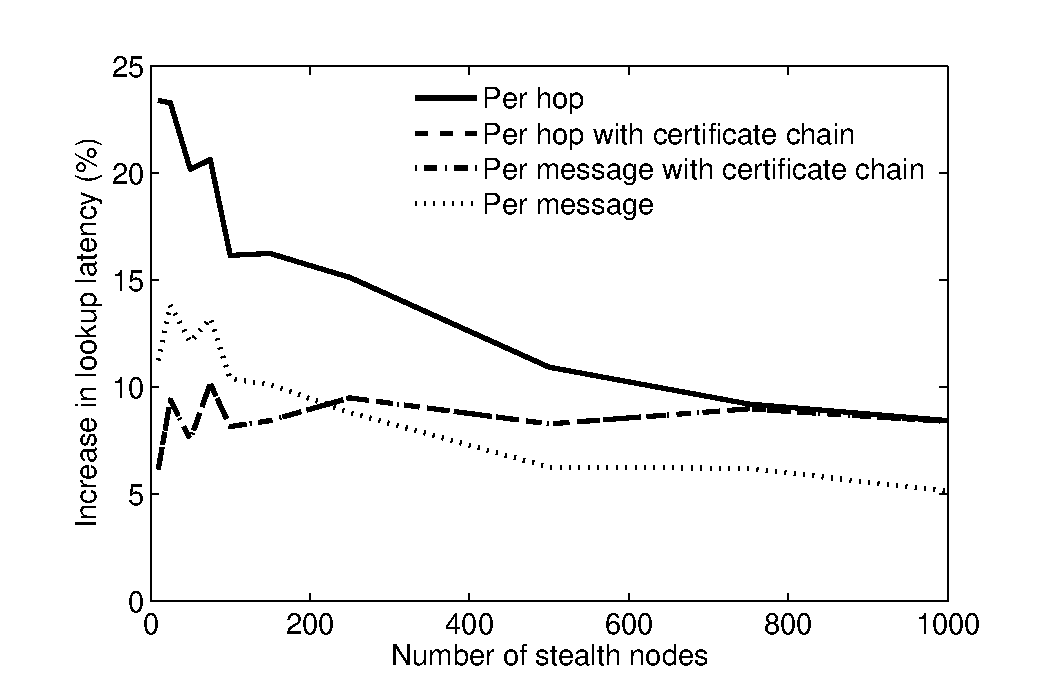
\includegraphics[width=0.5\textwidth]{./diagrams/Granularity2.eps}
    \label{fig-granularity2}}
\caption{\em Stealth DHT with 100 services nodes using an internal,
fully distributed PKI relative to a Stealth DHT with no authentication.
Note that the certificate-chain simulations are overlaid in these figures.}
\label{fig-granularities}
\end{figure}

Figs.~\ref{fig-granularities} show results for simulations conducted
with a fixed number of 100 service nodes, where the number of stealth
nodes was varied between 10 and 1000. The simulations were carried out
using our own discrete-event packet-level simulator, based on
Pastry~\cite{Rowstron01Pastry}. Each simulation was performed on a
GT-ITM~\cite{Calvert97Modeling} generated transit-stub topology of
1,000 routers, with 4\% transit nodes. Service, stealth and normal
Pastry nodes were connected to this topology in a random fashion.

Every service node in the DHT initially held its own certificate as
well as several content keys. During the simulation itself, stealth
nodes performed random \emph{get} requests for these keys at regular
intervals. Authentication was performed at the source and destination
in the \emph{per-message} results and also performed at each
intermediate node in the \emph{per-hop} results. For both cases,
simulations were run with and without certificate chains contained
within messages.

Fig.~\ref{fig-granularity} shows that both the per-hop and per-message
authentication schemes result in no increase in the overall number of
messages when certificate chaining is used. This is because all the
certificates required to fully authenticate a message's sender are
included within the message itself, thus increasing the average message
size, but resulting in no further requests to the CR.

On the other hand, an increase in the number of messages does exist
when certificate chains are not used. This increase is due to the
distributed nature of the Certificate Repository in an internal PKI; to
acquire a certificate in order to perform authentication, a node must
retrieve it from the service nodes through further DHT queries.
Expectedly, per-hop authentication results in markedly more messages
than per-message authentication. Also, as the number of stealth nodes
increases, the percentage increase in the number of messages relative
to a system without authentication falls. The reason for this is that
the increased number of stealth nodes results in an accordingly
increased number of requests for certificates. As all nodes cache
certificates upon receipt, there is no need for certificates to be
re-acquired.

Fig.~\ref{fig-granularity2} shows how lookup latency\footnote{The time
elapsed between a node requesting, receiving and fully verifying a key
from the DHT.} is affected by these factors. As expected, the cases
which involved querying the network (i.e. those without certificate
chains) result in increased lookup latencies. Note, however, that the
cases with certificate chains also incur increased lookup latencies
despite the lack of extra authentication messages. This is attributed
to the larger average message size that occurs as a result of including
certificate chains within messages.

As seen in Fig.~\ref{fig-granularity}, the relative increase in the
number of required authentication messages decreases with larger
numbers of stealth nodes. Fig.~\ref{fig-granularity2} therefore
displays a correlated reduction in lookup latency. As the cases with
certificate chains do not generate extra authentication message, they
remain unaffected by the number of stealth nodes in the DHT.

\SubSection{Permissions Management}
\label{subsect-permissions}

Managing the permissions of nodes on the network is yet another issue
with multiple solutions. One possibility is to simply place them within
each node's corresponding certificate, but this has two notable
associated issues. Firstly, certificates are immutable after they are
signed, so altering the permissions for a node would require a
certificate to be re-issued. Secondly, the average DHT message size
would have to increase to accommodate the larger certificates; exactly
how large they are depends on the volume of data required to represent
all the relevant details. However, such an approach does mean that the
relevant permissions are immediately available to any node receiving a
message containing the originating node's certificate. If per-node
permissions are not likely to change on a regular basis, this is
therefore a lower-overhead solution than using a separate certificate
repository.

An alternative approach would be to store permissions data within the
network somehow, thereby avoiding the lack of flexibility and larger
message sizes associated with storing them within certificates. The
inevitable cost, however, arises in the form of extra messaging
overhead; every time a node needs to check an individual's permissions,
they would have to look up and also validate the relevant data.

The permissions for a given node in a system such as those discussed in
this paper may require that some state is maintained for each
individual. For instance, this may be based on a record of how much in
the way of network resources or service usage the node has consumed. To
provide such functionality, an accounting mechanism of some sort is
therefore required.

%As with most of the issues discussed so far, there are numerous
%possible approaches to the problem of providing an accounting mechanism
%for nodes in a Stealth DHT, each with advantages and disadvantages.
%Nevertheless, the common goal of each is identical: to provide a system
%which offers ACID properties. These are \emph{Atomicity} (an action is
%either performed completely or not at all), \emph{Consistency} (an
%action cannot place the data in an invalid state), \emph{Isolation}
%(actions cannot interfere with each other's intermediate states) and
%\emph{Durability} (the result of an action will persist).
%
%The most straightforward approach is perhaps to just have a simple
%centralised server handle all transactions. This means messaging
%overhead is minimal, although it also means that a single point of
%failure exists for the system. Furthermore, dependent on the number of
%nodes considered, the server may be placed under load beyond its
%capabilities.
%
%Another possibility would be to improve load-balancing by distributing
%the transaction processing across multiple nodes. For instance, this
%could be achieved by mapping a given node's state to a key in the DHT.
%However, it is important to note that without replication, such a
%system would be prone to losing data from time to time. With
%replication, however, the management overhead required to maintain the
%aforementioned ACID properties will intuitively increase due to the
%need for agreement amongst the replicated nodes.
%
%The classical approaches for distributed accounting are divided into a
%few main categories, \emph{local accounting}, \emph{quorum-based} and
%\emph{token-based}. Local accounting refers to the case when nodes do
%not collaboratively maintain a count, but only keep values locally
%instead. In contrast, quorum-based systems require a group of nodes to
%maintain the count in a cooperative fashion~\cite{Castro99Practical}.
%Before the count is modified the quorum must reach a consensus on its
%old and new value. The more nodes that exist in the quorum the more
%robust the system is to malicious nodes and network failures.
%
%Token based
%systems~\cite{Liebau04Token}\cite{Thigpen02Distributed}\cite{Rivest96PayWord}
%may also use similar approaches, but the key difference is that each
%count is represented by many immutable tokens. Each token represents a
%currency that nodes can exchange for service. These tokens are
%cryptographically signed to restrict who can use them. Nodes acting as
%``banks'' may be used to store and certify the tokens to ensure that
%double spending does not take place. Tokens have the benefit that they
%can either be self-issued~\cite{Thigpen02Distributed}, or can be issued
%by the system~\cite{Rivest96PayWord}.
%
%Variations on mechanisms such as these may also be used to provide
%logging functionality in the DHT, thus making users accountable for
%their actions.

\SubSection{Certificate Revocation}
\label{subsect-revocation}

Invalidating a given certificate at an arbitrary point in time within
a PKI structure (\emph{i.e.} revoking it) is traditionally a difficult
problem, especially in distributed environments. However, the need for
the ability to revoke certificate often outweighs the cost of any
associated overhead. In other words, being able to remove a node from a
network before it can do any lasting damage may be worth the extra
associated costs. There are a number of possible methods for
certificate revocation, each with advantages and disadvantages (see
~\cite{Zheng03Tradeoffs}).

An obvious solution is for stealth nodes to be simply issued with
certificates with short expiration times, resulting in a
quasi-revocation scheme in which a CA can simply refuse to re-issue a
given certificate if it wishes to remove a given entity's privileges
within the system. Unfortunately, this intuitively has a high
maintenance overhead, as every individual that continues to exist on
the network will require a new certificate to be generated and issued
at a regular interval.

A common approach to this problem is to use a CRL, or Certificate
Revocation List. Any node verifying a certificate must then check the
list as part of its normal authentication process. The list itself may
be stored in one of a number of ways. For instance, and as with many of
the other issues considered so far, a centralised server could be used.
Again, the problems common to this sort of approach are that it creates
a central point of failure, and could potentially result in the
overloading of the server if many requests are regularly made. A
distributed approach amongst service nodes could potentially be used to
alleviate the load placed upon any one node, but this results in
increased messaging overhead due to the added complexity of maintaining
and retrieving the list. It is important to note that, of course, the
list may be kept in its entirety on multiple nodes as well as the
approach of splitting it amongst them (\emph{i.e.} replication vs.
division, respectively).

%There also exist several approaches for the manner in which nodes
%access such lists. In general terms, these fall into the \emph{pull}
%and \emph{push} distribution models. As an example of the pull model,
%nodes may poll the holder(s) of the CRL at regular intervals, or even
%for every transaction, depending on the level of granularity required.
%An example of the push model would be the Certificate Revocation List
%being broadcast to all nodes upon any update, or at a regular interval.
%Obviously, such an approach may result in a great deal of
%initialisation overhead if a large number of nodes which require the
%CRL exist; multicast overlays may have to be built, and ideally with
%some method of guaranteeing delivery. For small numbers of nodes,
%however, the cost of broadcasting updates and/or occasionally
%broadcasting the full list may be lower than having nodes repeatedly
%request it unnecessarily.

\Section{Related Work}
\label{sect-related}

Many previous works have discussed the varied problems associated with
untrustworthy nodes in DHTs, noting that security is an issue commonly
overlooked in algorithm proposals. For example, \cite{Sit02Security}
and \cite{Castro02Secure} both discuss possible DHT attacks and
defenses. In the former, Sit and Morris broadly define three types of
malicious behaviour: routing, storage and other miscellaneous attacks.

A commonly encountered technique often used in all three categories is
the ``Sybil'' attack, as originally described by Douceur
in~\cite{Douceur02Sybil}. This refers to the situation when a single
malicious node is able to masquerade as multiple distinct entities
within the network in order to gain control of a substantial fraction
of it. The conclusion is drawn that a suitable defense against such an
attack is to have a logically centralised authority which is capable of
certifying the identity of nodes in the network. Therefore, this work
can be said to support our approach of implementing a PKI in
conjunction with a Stealth DHT.

Routing attacks in a DHT may refer to nodes deliberately providing
incorrect lookups or producing incorrect routing updates. More
specifically, an example could be the ``Eclipse'' strategy, as
discussed in detail by Singh \emph{et al.} in~\cite{Singh06Eclipse}.
This involves multiple malicious nodes deliberately attempting to
partition peer-to-peer overlays in a form of Distributed Denial of
Service (DDoS) attack. Again, the suggestion is made of a certification
scheme as a straightforward solution, as with our approach to such a
problem. Beyond this, the authors propose defenses such as constraining
the entries placed in routing tables~\cite{Castro02Secure} or
periodically auditing the connectivity of other nodes to detect
anomalies which are symptomatic of those conducting such an attack.

Storage attacks may involve behaviour such as nodes refusing to store
objects, corrupting them or simply denying their existence. More
resourceful attackers may also use multiple malicious nodes to attempt
to take control of specific pieces of content. Some may even try to
make it impossible to access useful content by flooding the network
with useless data~\cite{Liang06Index}. Srivatsa and Liu suggested the
approach to obfuscate the location on the DHT of specific keys from
those not authorised to access them~\cite{Srivatsa05Countering},
although the most commonly suggested solution is to make use of some
sort of digital certification scheme, such as the one we have proposed
in this paper. Furthermore, a Stealth DHT can ensure that potentially
untrustworthy nodes are never even part of the DHT which is responsible
for storing keys, although they may still access them if authorised to
do so.

Of course, DHT-based storage systems have often considered security in
their own right. PAST, for instance, uses the concept of
``smartcards'', with which users hold associated public/private
keys~\cite{Druschel01PAST}. These smartcards are managed by brokers
(trusted third parties). In other words, PAST is yet another system
that takes the approach of using a Public Key Infrastructure for
security purposes; again, the concept we have suggested and expanded
upon in this paper.

In terms of miscellaneous attacks, Sit and Morris also noted that an
attacker may attempt to conduct a DDoS attack by causing multiple nodes
under their control to rapidly join and leave the network, resulting in
degradation of DHT
performance~\cite{Rhea04Handling}\cite{Li04Comparing}. Possible
solutions to this problem are suggested in~\cite{Castro02Secure}, such
as forcing nodes to solve crypto-puzzles before they may join as a
means of slowing down attackers attempting to run multiple logical
nodes on a single physical machine. However, such an approach merely
makes carrying out an attack slightly more difficult. Our Stealth DHT
approach, however, means that stealth node churn has a significantly
reduced effect on DHT performance relative to nodes churning in
traditional DHTs.

Several works have also considered how such authentication systems may
be implemented in a physically distributed fashion over peer-to-peer
networks. For example, Aberer \emph{et al.} discussed how a completely
decentralised PKI based on a statistical approach could be deployed on
many traditional DHTs (although they specifically use
P-Grid~\cite{Plaxton97Accessing})~\cite{Aberer04Decentralized}. The key
difference in comparison with our work is that in this case, the
authors consider a method that can function with a network consisting
entirely of potentially untrustworthy nodes. However, they note that
their system breaks down if more than 25\% of nodes are actually
malicious, and that it may not function with several DHTs, such as CAN
or Chord~\cite{Ratnasamy01Scalable}\cite{Stoica01Chord}. We, however,
believe that our system is implementable on any existing DHT, and
should function regardless of the percentage of malicious stealth
nodes.

\Section{Conclusion}
\label{sect-conclusion}

The original goal of our Stealth DHT proposal
was to provide a distinction between nodes of greater and lesser
capabilities as a means of improving routing performance. Powerful
nodes were responsible for handling message forwarding within the DHT,
whereas the remaining, weaker nodes simply requested services from
them. In this paper, we have shown that this separation can be extended
to incorporate both verifiably trustworthy and potentially
untrustworthy nodes. By selectively limiting the privileges of
untrustworthy nodes on the network, on an individual basis if required,
we can accordingly limit the numerous security problems associated with
supplying service to them. By further augmenting our approach with a
suitable Public Key Infrastructure to enforce the separation between
node types, we have shown how a Stealth DHT can be used to supply a
secure, resilient overlay that caters to both trustworthy and
untrustworthy nodes simultaneously. Stealth DHTs do not necessarily
need to deny access to potentially untrustworthy nodes as opposed to
previous approaches that addressed security issues in DHTs. Instead,
Stealth DHTs only limit the operations that such nodes can perform.
Further to this, we have discussed a number of issues and possible
solutions related to implementing a PKI in a Stealth DHT.

In the future, we intend to add provisions for node authentication
in our existing Stealth DHT implementation, so that it may be
evaluated in a real-world environment.

\bibliographystyle{latex8}
\bibliography{auth}

\end{document}
